% Template for ICIP-2018 paper; to be used with:
%          spconf.sty  - ICASSP/ICIP LaTeX style file, and
%          IEEEbib.bst - IEEE bibliography style file.
% --------------------------------------------------------------------------
\documentclass{article}


\usepackage{spconf,amsmath,graphicx}
\usepackage{epstopdf}
\usepackage{amssymb}


\usepackage[linesnumbered,ruled,vlined]{algorithm2e}
\usepackage{algpseudocode}
\usepackage{amsmath}

\usepackage{color}
\renewcommand{\algorithmicrequire}{\textbf{Input:}}
\renewcommand{\algorithmicensure}{\textbf{Output:}}



\newcommand{\comments}[1]{}
\newcommand{\cxj}[1]{\textcolor[rgb]{1.00,0.00,0.00}{(xuejin:#1)}}
\newcommand{\xjmd}[1]{\textcolor[rgb]{0.00,0.00,1.00}{#1}}

%%%% definitions
\newcommand{\ptset} {\mathbb{P}}

\makeatletter
    \newcommand\fcaption{\def\@captype{figure}\caption}
\makeatother
% Example definitions.
% --------------------
\def\x{{\mathbf x}}
\def\L{{\cal L}}

% Title.
% ------
\title{SKETCHPOINTNET: Learn to recognize sketches as time serieses}
%
% Single address.
% ---------------
\name{Paper XXX}
\address{ }
%
% For example:
% ------------
%\address{School\\
%	Department\\
%	Address}
%
% Two addresses (uncomment and modify for two-address case).
% ----------------------------------------------------------
%\twoauthors
%  {A. Author-one, B. Author-two\sthanks{Thanks to XYZ agency for funding.}}
%	{School A-B\\
%	Department A-B\\
%	Address A-B}
%  {C. Author-three, D. Author-four\sthanks{The fourth author performed the work
%	while at ...}}
%	{School C-D\\
%	Department C-D\\
%	Address C-D}
%
\begin{document}
%\ninept
%
\maketitle
%
\begin{abstract}
Sketch recognition has been studied for years. In previous works, sketches are only treated as images, which ignores the sparse nature of sketches. In this paper, we retreat each sketch as a series of track points and propose a neural network to recognize it. Our network, termed as SketchPointNet, achieves the highest recognition accuracy among point-based sketch recognition approaches. We use a novel group scheme which investigates the timing characteristic of sketch points, which ensures the integrity of local patterns. SketchPointNet needs very few parameters compared with image-based sketch recognition approaches. Meanwhile, it still achieves a high recognition accuracy which is close to the state-of-the-art approaches on TU-Berlin dataset.
\end{abstract}

\begin{keywords}
Point-based sketch recognition, parameters, image-based sketch recognition, SketchPointNet, recognition accuracy
\end{keywords}

\section{Introduction}
\label{sec:intro}

With the popularity of mobile and potable devices, people are getting easier to sketch objects. Sketches have proved to be a powerful and effective tool for communication. A mount of approaches focused on sketch recognition have been studied. But all of them take the recognition accuracy as their only benchmark with ignorance of recognition speed. Mobile and portable devices have more limited computing resources and storage compared to high-performance server or even personal computer. So it is necessary to promote the speed of sketch recognition, but not only accuracy.

Although sketches and images can be visually recognized, they have two main differences: (i) Patterns take more important place in sketch recognition than in image recognition. Sketches vary largely within class. Meanwhile, some sketches coming from different class have similar looking from the high level. But differences can be told from the mid level or low level, e.g., some cats and snowmen are identified easily from their facial part, but hardly from the whole sketches. Objects in images are from the real life. The size of different parts from one object in images are more rationale than that in sketches. (ii) Sketches are sparser than images. Sketches are composed of a group of strokes. For a sketch, most area is blank. Images contains richer information such as texture and dilation. (iii) Sketches have time information. They are generated from a pen. This means a sketch can be viewed as a series of points.

Previous works on sketch recognition are generally borrowed from image classification paradigm. Both conventional sketch recognition and Deep Neural Networks (DNNs) take sketches as images. These methods do not take full advantage of the sparsity of sketches. Besides, in pursuit of high accuracy, they developed different feature fusion methods without the consideration of the model is too bloated to be distributed in mobile devices. Due to special generalization a sketch, it can be represented by only a series of points which takes less storage than represented as an image.

\textbf{Traditional sketch recognition.} In early years, sketch recognition applications \cite{Hse2004SketchedSR, LaViola2004MathPad2AS, Fonseca2000UsingFL} are mainly used for letters and numbers. Hse and Newton \cite{Hse2004SketchedSR} use Zernike moments as features for sketches. Laviola et al. \cite{LaViola2004MathPad2AS} develop an approach for common mathematical symbols recognition. Fonseca and Jorge \cite{Fonseca2000UsingFL} design geometrical features  according to profiles of stokes. These approaches achieve good results because of the simplicity of the symbols.

Symbols from the same class usually have a standard template. Eitz et al. \cite{Eitz2012HowDH} publish a largely free-hand drawn sketches dataset TU-Berlin including common 250 categories of objects. All the objects from same class are drawn by the impression. There are huge difference in class. Eitz et al. extract HOG features of sketches and use a support vector machine(SVM) for classification. Other existing traditional works \cite{LiHSG15, Schneider2014SketchCA} also extract hand-crafted features and use SVMs for classification. The results of traditional approaches are not good on this challenging dataset, for which, humans only acheive 73.1\% recognition accuracy.

\textbf{DNN-based sketch recognition.} DNN-based approaches have greatly boosted image recognition performance. Sketch-a-Net \cite{Yu2015SketchaNetTB} and DeepSketch \cite{Seddati2015DeepSketchDC} are both proposed deep Convolutional Networks (ConvNets) for sketch recognition. Both of them are derived from image recognition ConvNets. They have larger convolutional kernel size and less convolutional layer compared with general image recognition ConvNets.

Although Sketch-a-Net \cite{Yu2015SketchaNetTB} and DeepSketch \cite{Seddati2015DeepSketchDC} achieve higher recognition accuracy than traditional methods. They still treat each sketch as an image, which do not take full advantages of sparsity of sketches.

\textbf{Point-based 3d model recognition} takes 3d model as group of unordered points. Sketches and 3d models are both a group of points. The difference is: (i)sketches are group of 2d points instead 3d points; (ii) sketch points have time information for they are generated from a pen.

PointNet \cite{qi2017pointnet} summarises the critical points for each class. This ignores the patterns of 3d models. PointNet++ \cite{qi2017pointnetplusplus} uses a hierarchical architecture to summarise patterns of 3d model gradually. Sketches have time information for each points, which shows the way of sketches being generated.

Li et al. \cite{1801.07791} use farthest point sampling to select representative points and  aggregate the $K$ closest points around the representative points. Then they use $\chi$-Conv to extract local features gradually. One of the most time-consuming step is that they have to use multilayer perceptron on the whole local points.

In this paper, we propose a DNN, SketchPointNet, for accelerating sketch recognition and reducing recognition model size, which derived from PointNet \cite{qi2017pointnet}. Comparing with existing DNN-based sketch recognition approaches, we treat each sketch as a series of points which is a sparser representation than image. PointNet++ \cite{qi2017pointnetplusplus} summarize patterns in 3d space, while ours summarize pattern in 2d space. Besides, we incorporate each points of sketches with stroke order information which is unique for sketch points. SketchPointNet is designed with two notable characteristics: (i) a group of micro PointNets are encoded in SketchPointNet hierarchically to capture features of different level; and (ii) micro PointNets summarize patterns along the time series points, while image-based DNN's kernels move in two directions.

Our contributions are summarized as follows: (i)for the first time, we take sketches as a series of points and propose a corresponding DNN to recognize them; (ii) we demonstrate that SketchPointNet has a higher recognition speed and a smaller model size than existing DNN-based approaches.



\section{Methodology}
\label{sec:methodology}

In this section, we will first introduce the network architecture of our SketchPointNet. Next, we describe the algorithm details of point sampling and grouping from sketch strokes, as well as the network to extract both local and global patterns for recognition.


%\subsection{Architecture of SketchPointNet}
%\label{ssec:sketch_point_net}
%\vspace{0.15cm}
\para{Architecture of SketchPointNet.}
Fig.~\ref{fig:sketchpointnet} shows the architecture of our SketchPointNet.
%
The directly captured stroke paths from various input devices are typically contact points that distribute unevenly along strokes with different movement speeds and device sizes.
To make them directly comparable, we resample the input sketch $\mathcal{S}$ into $N$ evenly distributed points as a point set $\mathbb{P}=\{P_i|i=1,\ldots,N\}$.
%Moreover, the current Tensorflow only supports static graphs. Resampling the input sketch into a fixed number of points makes the implementation simple.
A transformation net is firstly employed to regress a transformation matrix to align the input sketch, similar with PointNet~\cite{qi2017pointnetplusplus}.
%
Given the resampled and transformed point set, we extract the sketch features hierarchically with three mini PointNets~(PN-1, PN-2, PN-3) from the lower level to the global level.
%
In each level, we group the point set $\ptset$ into $K_g$ groups according to their spatial and temporal neighborhood in different size.
Stroke features are extracted using a mini PointNet~\cite{qi2017pointnetplusplus} for each point group.
%
From the global pattern extracted and used to predict the scores for the $N_{class}$ sketch categories in the third PointNet (PN-3).


While the overall architecture of our SketchPointNet is similar with PointNet++~\cite{qi2017pointnetplusplus}, the main difference lies on the sampling and grouping procedure.
Targeting at 3D point clouds, PointNet++~\cite{qi2017pointnetplusplus} considers the spatial distribution of points in the 3D space.
In contrast, not only the spatial pattern is important, the temporal pattern is also important for sketch recognition.
%
During our sampling and grouping, the temporal and spatial information is integrated together to extract sketch features for robust recognition.


%\subsection{Point Sampling}
%\label{ssec:resample}
%\vspace{0.15cm}
\para{Point sampling.}
%% key concept of resampling is to preserve local temporal and spatial relations
To make various sketches comparable, we sample $N_{pt}$ equidistantly spaced points along strokes.
By sampling along strokes, the temporal information is encoded in the point distribution.
%
The length of each stroke is calculated and the total length of all strokes is $L_{sum}=\sum^{M}_{i=1} L_i$, where $M$ is the stroke number.
%
Given the desired point number $N_{pt}$, we assign each stroke $N_i=\frac{L_i}{L_{sum}}N_{pt}$ points according to its stroke length $L_i$.
Then we reample each stroke into $B_i$ points equidistantly along the stroke.
%
Fig.~\ref{fig:resample} shows the sampling results with different number of points.
We can see that the main structure is well preserved during the sampling procedure without losing much details, even with a very small number (N=128) of points.

\begin{figure}
	\center
	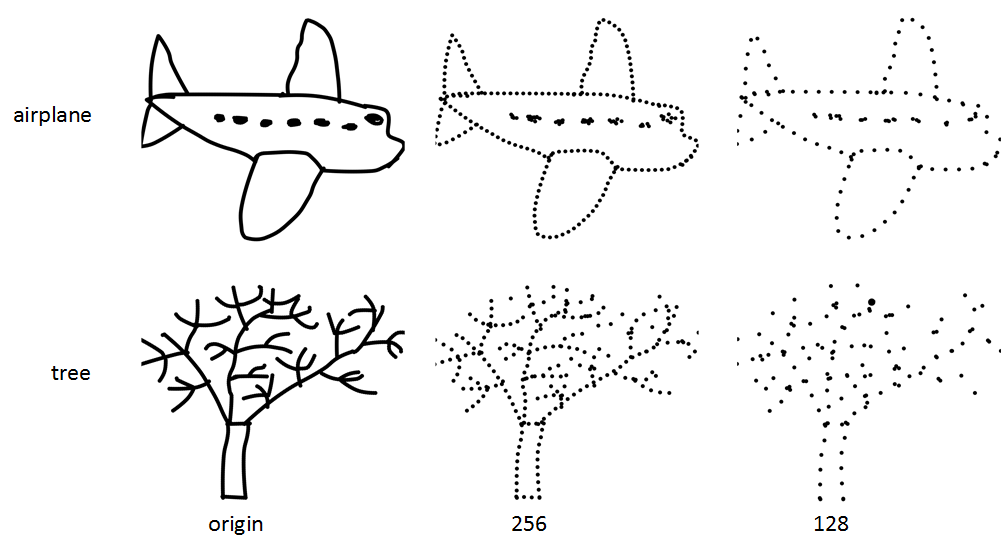
\includegraphics[width=3in]{images/resample2.png}
	\fcaption{Sketch resampling with different number of points. Each continuous stroke is shown in a unique color.}
	\label{fig:resample}
\end{figure}



%\subsection{Point Grouping}
%\label{ssec:group_scheme}
%\vspace{0.15cm}
\para{Point grouping.}
To extract features of the input sketch, we group a set of points on the strokes and feed them into a mini PointNet, which is flexible with the number of input points.
%
Given a desired number of groups $N_{group}$ at a certain level, we first sample $N_{group}$ points from the input sketch as the group centers using the sampling method described above.
%
Then, for each group, we extract a set of points equidistantly on the input strokes in an area of radius $r$ surrounding the group center.
%
The number $K_{group}$ of points in different groups varies over the sketch region. We set an upper bound for $K_{group}$ to reduce the computational complexity.
%While the sketch is first re-sampled evenly distributed temporarily in the previous sampling step, the point density is not even in the spatial domain.
%We sample the partial sketch in a local region to a number $K_{group}$ of points equidistantly.
%
As Fig.~\ref{fig:group} shows, the points in a local region with different radius present different local patterns.
%
By sampling points along strokes, both temporal and spatial patterns are preserved during the grouping procedure, which are essential for sketch recognition.


\begin{figure}
	\centering
	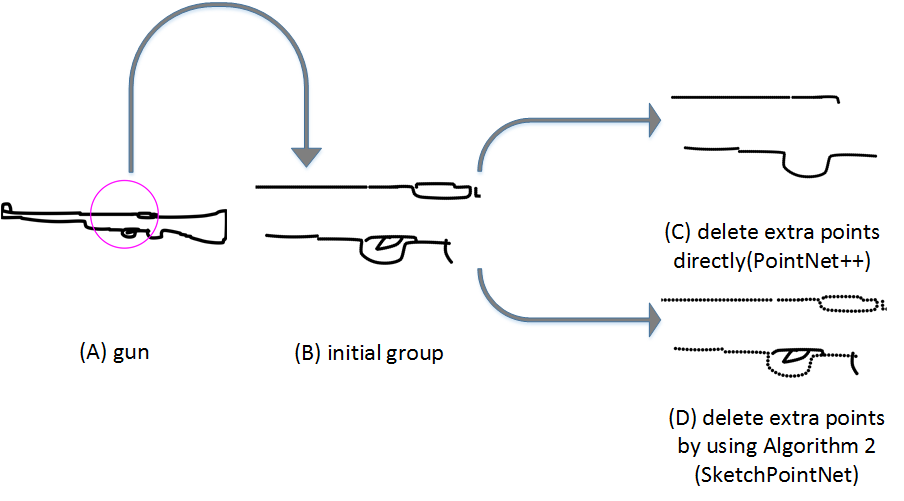
\includegraphics[width=\columnwidth]{images/group.png}
	\fcaption{By grouping points in local regions of different radious $r$, features of different level are extracted. The middle and right columns show the sampled points with different number of points $K_g$ in a local region.   }
	\label{fig:group}
\end{figure}

\begin{figure}
	\centering
	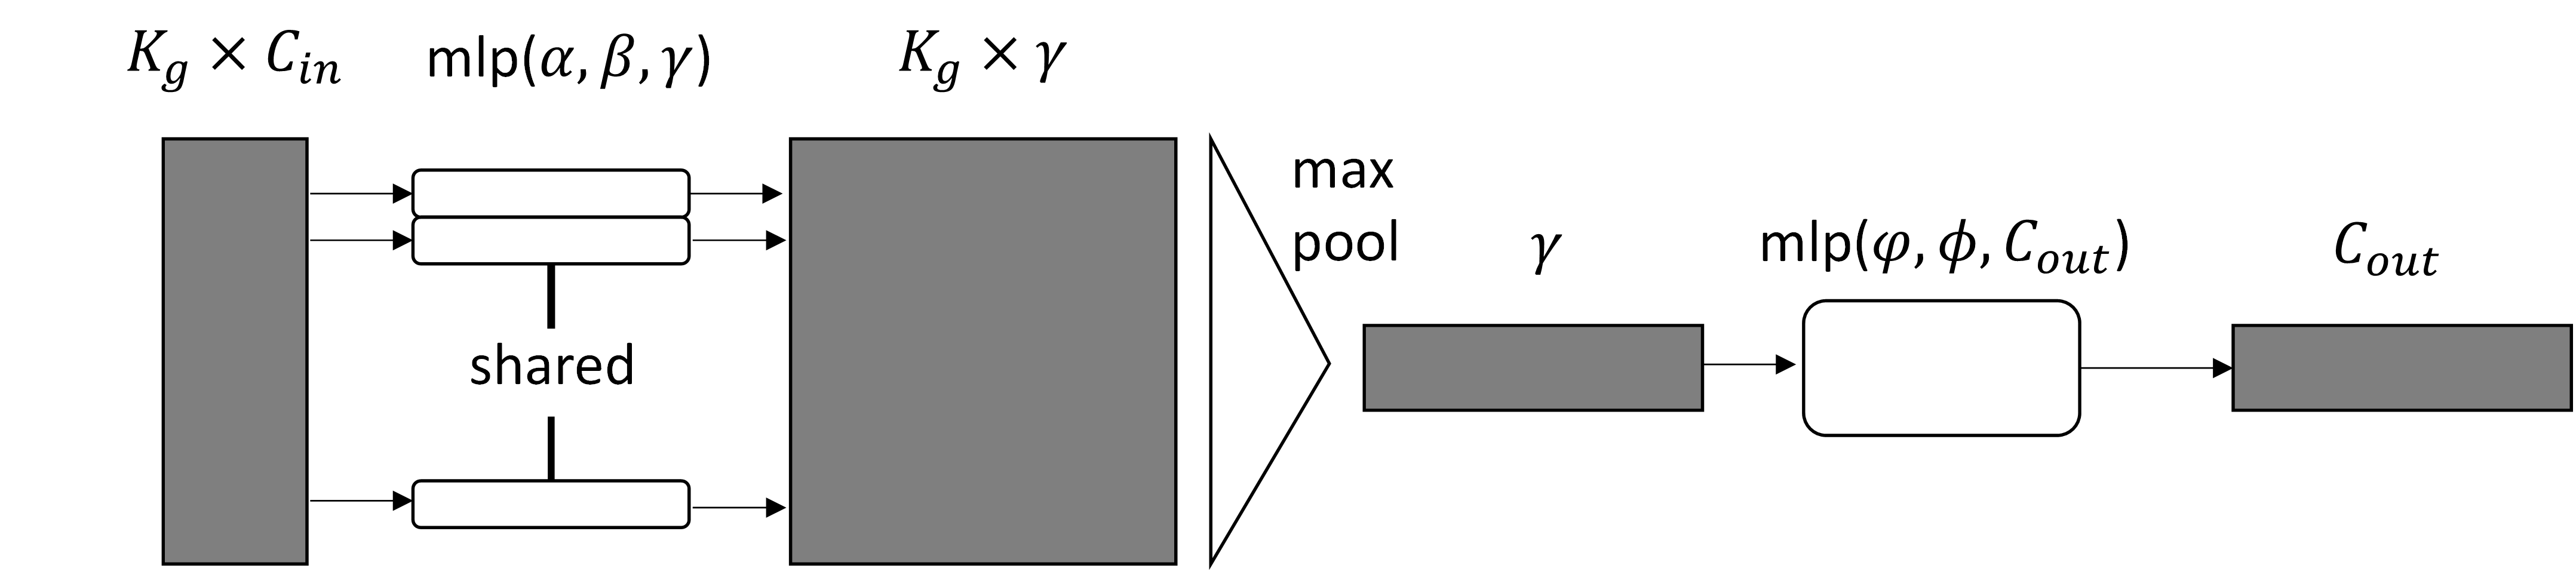
\includegraphics[width=\columnwidth]{images/pointnet.png}
	\caption{Architecture of our mini PointNet.}
	\label{fig:miniPN}
\end{figure}
%\subsection{Group Pattern Extraction}

%\vspace{0.15cm}
\para{Pattern extraction.}
%
We use a modified version of the PointNet~\cite{qi2017pointnet} to extract the sketch pattern in a local region that contains various number of points.
The architecture of our mini PointNet is shown in Fig.~\ref{fig:miniPN}.
%
%After the point grouping step, we feed a mini PointNet with $N_g$ groups with data size $N_g \times K_g \times C$ to extract the sketch pattern for recognition.
%
For each group, a mini PointNet is fed with $K_g$ points in its local region with data size $K_g \times C_{in}$.
$C_{in}$ is the number of data channel of each point.
Each mini PointNet consists three parts.
The first part is $K_g$ shared-weight three-layer perceptrons (with $M^{1}_1$,$M^{1}_2$,$M^{1}_3$ neurons at each layer respectively), which converts the input data of each point into another feature space.
%
The second part is a max-pooling layer to aggregate features of the $K_g$ points into a fixed-dimension feature.
%
The third part is a three-layer perceptron (with $M^{2}_1$,$M^{2}_2$,$M^{2}_3$ neurons at each layer respectively).
%
The output of the mini PointNet is a $C_{out}=M^{2}_3$ dimensional feature vector.
%Here, $N_g$ is the number of local groups, $K_g$ is the number of points in each group, $C$ is the number of data channel of each point.


Initially, we have the 2{D} coordinates and stroke order of each point for the normalized sketch.
We translate each point into a local frame relative to the center point of each group.
Therefore, the data channel $C^1_{in}=2+1$ for the first PointNet PN-1, including the 2D local coordinates and 1-D stroke order.
The output of PN-1 is a $C^1_{out}$ dimensional feature vector for each group.
%
Different with PointNet++~\cite{qi2017pointnetplusplus} for 3D point clouds, the stroke order does matters for sketch recognition, because human typically draw the overall shape and then add fine details later.
%
The strokes drawn earlier have more impact effects for recognizing a coarse sketch.
%

Then, increasing the radius $r_2$ for grouping points, which is equivalent to increasing the receptive field, we extract sketch patterns in a higher level.
%
For the second PointNet PN-2, the input is the $K_{g2} \times C^2_{in}$ data, where $K_{g2}$ is the number of points in the local region of a group, $C^2_{in}=2+1+C^1_{out}$ for each group, including the 2-D local coordinate of the group center, 1-D stroke order and the $C^1_{out}$-D feature extracted for the local region from the first PointNet.
%
The output of PN-2 is a $C^2_{out}$-D feature vector for each group.

%\vspace{0.15cm}
\para{Sketch classification.}
%\label{ssec:classification}
After the two-level local pattern extraction, we feed the $N_{g2} \times C^2_{out}$ data into the third mini PointNet PN-3, which produces $C^{3}_{out}=N_{class}$ dimensional vector as the predicted scores for the $N_{class}$ categories.





\section{Experiments}
\label{sec:experiments}
In this section, we evaluate our method using  TU-Berlin sketch benchmark. It contains 250 classes. Each class has 80 instances. We do a group of experiments to compare our method with other methods in recognition speed and accuracy. Like previous works, we use 3-fold cross-validation within the dataset.


\subsection{Recognition accuracy with different $N$}
\label{ssec:resample_number}

From the Fig.~\ref{fig:resample}, we can see that 1024 points are enough to represent a tree. 512 points can also represent a tree but a little sparser. Even a tree with 256 points are visually clear for humans. In order find a proper $N$, we did a group experiments with $N = 1024, 512, 256, 128$. If $N$ is too large, there are no good for recognition accuracy, but makes recognition speed slower.

\begin{table}[htbp]
\begin{tabular}{|p{1.4cm}|p{1.3cm}|p{1.3cm}|p{1.3cm}|p{1.3cm}|}
    \hline
     $N$ & 1024& 512 & 256 & 128\\
    \hline
     accuracy & x\% & x\% & x\%& x\%\\
    \hline
\end{tabular}
\caption{Classification with different $N$.}
\end{table}

\subsection{Comparison of different methods in recognition speed and accuracy}
\label{ssec:cm_speed}
SketchPointNet is derived from PointNet. It uses lots of shared architecture, which means less parameters compared with existing Image-based sketch recognition approaches. We performed Sketch-a-Net(vallina), DeepSketch 1 and SketchPointNet on Titan 1080 with tensorflow 1.2. The whole model of Sketch-a-Net and DeepSketch 2 \cite{Dupont2016DeepSketch2D} use different feature fusion method, which makes the whole models too large to suite the mobile computing device. So we only compare 3 end-to-end networks(Sketch-a-Net(vallina), DeepSketch 1 and SketchPointNet).

\begin{table}[htbp]
\centering
\begin{tabular}{cccc}
    \hline
     -&Sketch-a-Net& DeepSketch& Ours\\
    \hline
     model size& 64M&223M& 33M\\
     speed &10.92ms&10.6ms& 5.2ms\\
     accuracy & 72.6\% & 75.6\%& x\% \\
    \hline
\end{tabular}
\caption{Performance comparison of different networks.}
\label{tbl:speed}
\end{table}
From the tabel ~\ref{tbl:speed} we can see that our model is faster and smaller than Sketch-a-Net(vallina) and DeepSketch 1. Although our model are smaller compared with existing DNN-based appraches. We still achieve a high recognition accuracy.

\begin{table}[htbp]
\centering
\begin{tabular}{ll}
    \hline
     models &accuracy\\
    \hline
     HOG-SVM (Eitz et al, 2012)& 56\%\\
     Ensemble (Li et al, 2013) &61.5\%\\
     MKL-SVM (Li et al, 2015) & 65.8\% \\
     FV-SP (Schneider and Tuytelaars, 2014) & 68.9\% \\
     LeNet (LeCun et al, 2012)& 55.2\% \\
     Sketch-a-Net(vallina)(Yu et al, 2015)& 72.6\% \\
     Sketch-a-Net(Yu et al, 2016)& 77.95\% \\
     DeepSketch 1(Seddati et al, 2015)& 75.42\% \\
     DeepSketch 2(Seddati et al, 2016)& 77.69\% \\
     Our Model& x\% \\
    \hline
\end{tabular}
\caption{Sketch recognition with different models.}
\label{tbl:acc}
\end{table}

\section{Conclusion}
\label{sec:conclusion}

In this paper, we propose SketchPointNet, a compact deep neural network for robust sketch recognition.
%
Our network directly consumes 2D points on freehand sketches, which are sparsely distributed in the 2D space.
%
By sampling and grouping points while considering both temporal order and spatial distribution, local features are learned hierarchically using three mini PointNets.
%
The experiments on the challenging TU-Berlin dataset demonstrated that our SketchPointNet achieves a high recognition accuracy, and significantly reduces the number of network parameters.
%

\noindent \textbf{Acknowledgements.} This work was supported by the National Key Research \& Development Plan of China under Grant No. 2016YFB1001402�� and the National Natural Science Foundation of China under Grants. 61472377, 61632006, 61331017,61622211, and 61472392.

\bibliographystyle{IEEEbib}
\bibliography{strings,refs}

\end{document}
